\Chapter{Servicios básicos}{UDP y TCP}
\section{Programación de red: UDP}
\subsection{Módulos de ayuda}
Para esta práctica, se desarrollan módulos de Python que faciliten las tareas básicas,
como lecturas de hosts y puertos por argumentos: \\
\begin{minipage}{\linewidth}
	\centering
	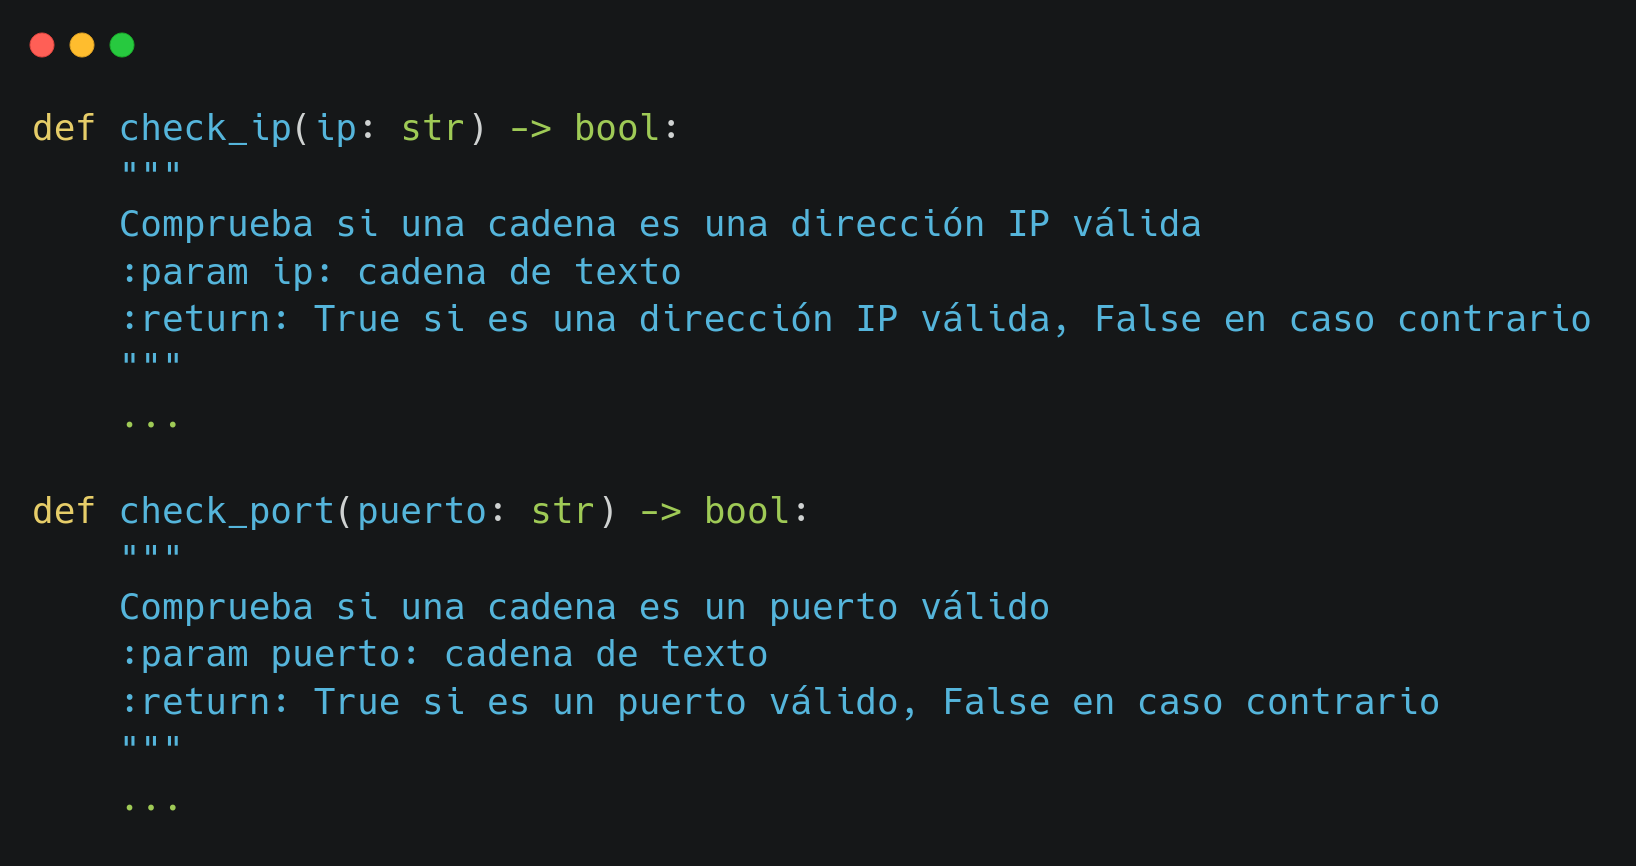
\includegraphics[width=1\textwidth]{1/code1.png}
	\captionof{figure}{Estructura del módulo de ayuda ``ips.py''}\label{fig:1/code1}
\end{minipage}
\\
\begin{minipage}{\linewidth}
	\centering
	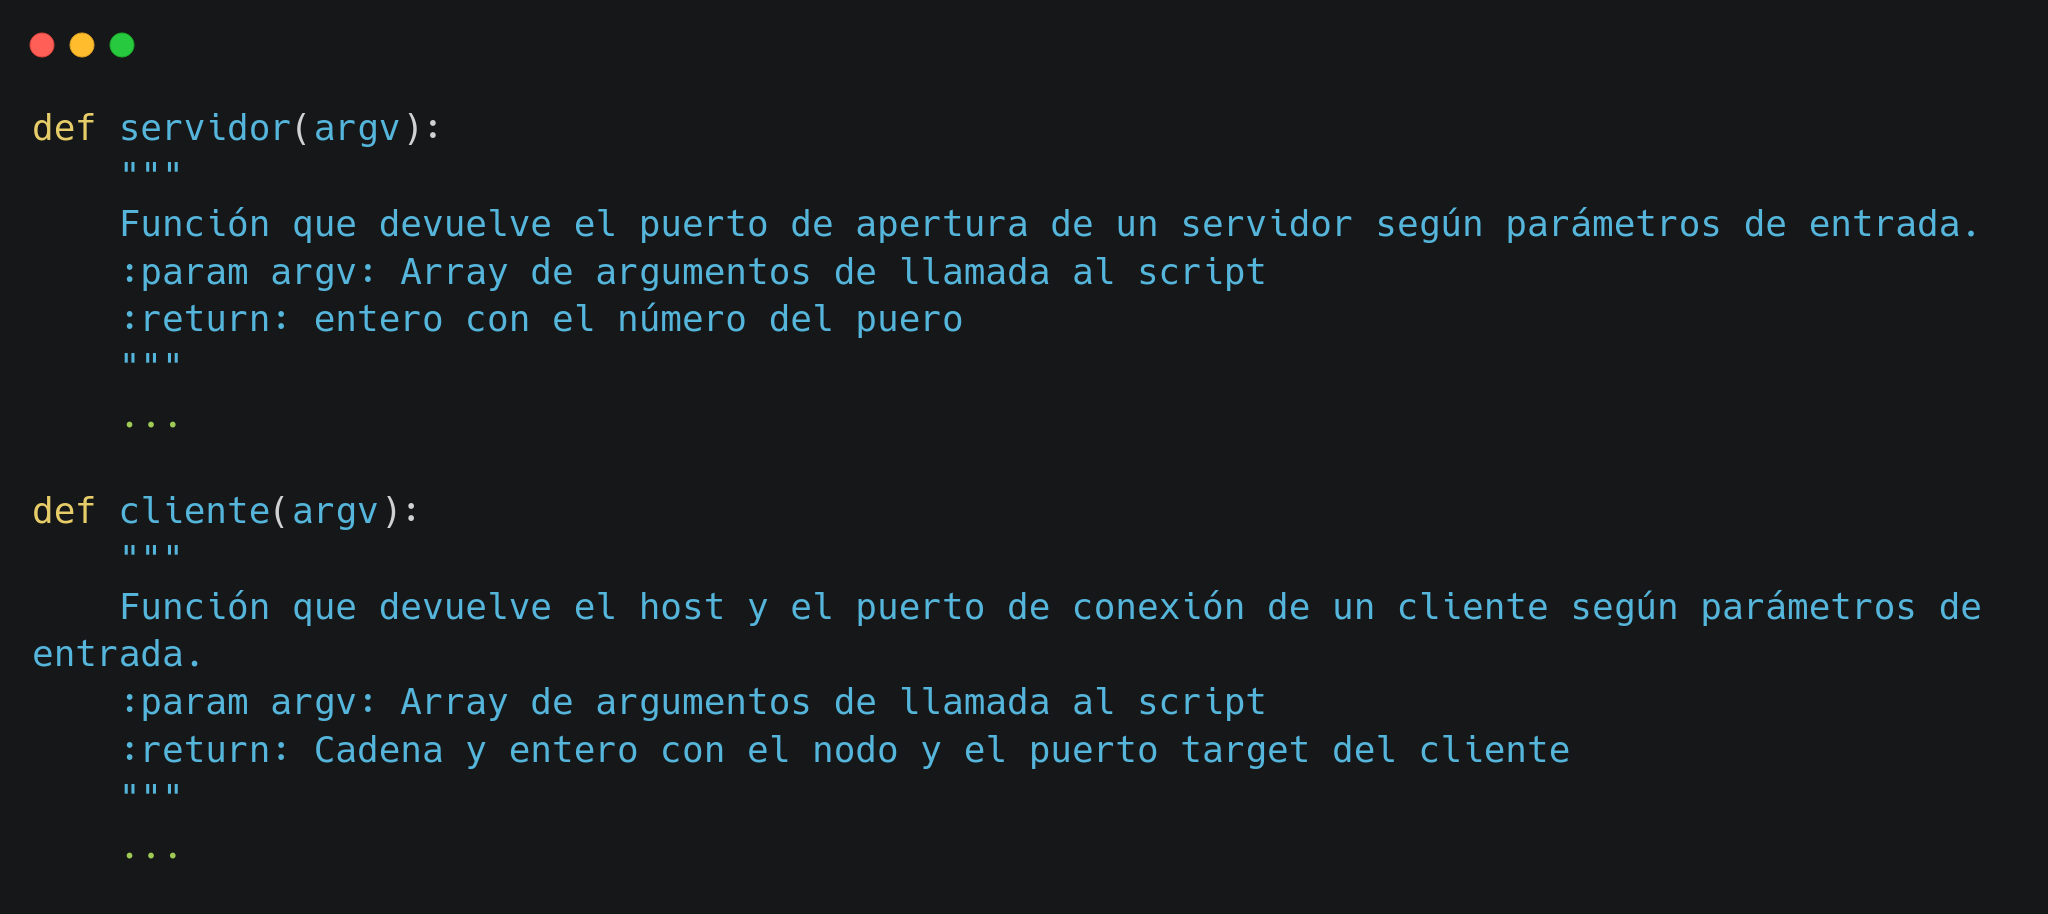
\includegraphics[width=1\textwidth]{1/code2.png}
	\captionof{figure}{Estructura del módulo de ayuda ``ips\_argv.py''}\label{fig:1/code2}
\end{minipage}

\subsection{Ejercicio 1}

\subsection{Ejercicio 2}

\subsection{Ejercicio 3}

\subsection{Ejercicio 4}

\section{Programación de red: TCP}
\subsection{Módulos de ayuda}
Se reutilizan los módulos de la sesión anterior (\ref{fig:1/code1}~y~\ref{fig:1/code2}) para
realizar todos los ejercicios. Además, para los ejercicios ``oche'' se reutiliza el código
usando otro módulo nuevo: \\
\begin{minipage}{\linewidth}
	\centering
	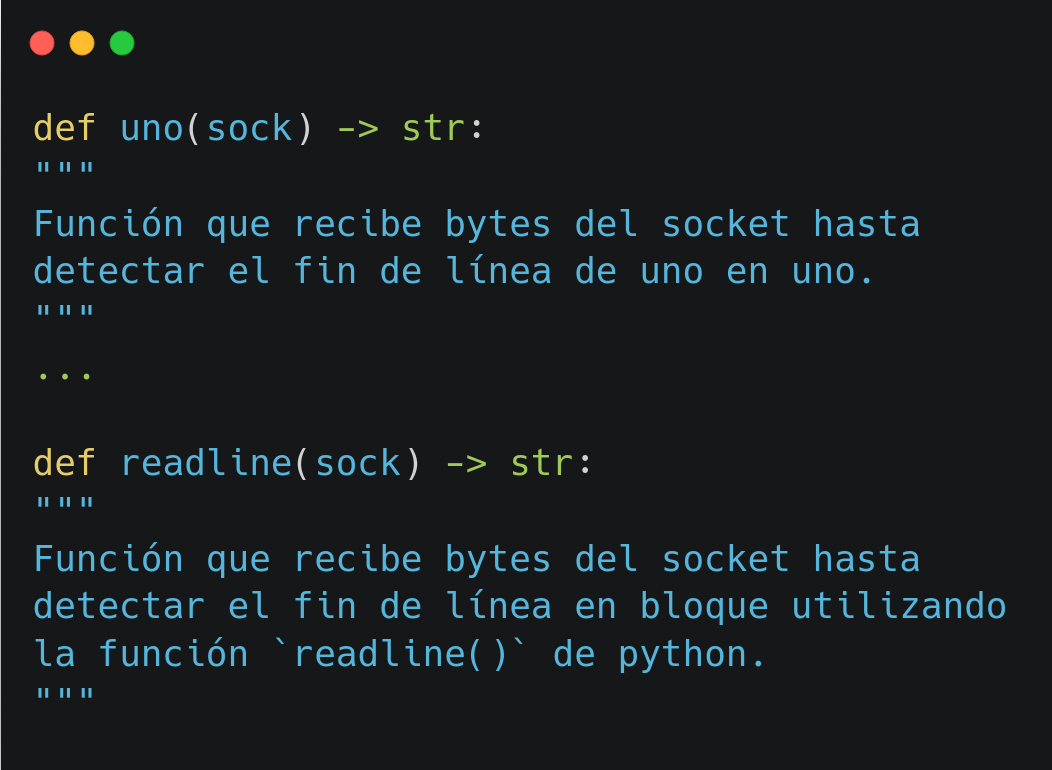
\includegraphics[width=1\textwidth]{1/code3.png}
	\captionof{figure}{Estructura del módulo de ayuda ``recibir\_mensaje.py''}\label{fig:1/code3}
\end{minipage}

\subsection{Ejercicio 1}

\subsection{Ejercicio 2}

\subsection{Experimento}

\subsection{Ejercicio 3 / Experimento}

\subsection{Ejercicio 4 / Experimento}

\subsection{Ejercicio 5}

\subsection{Ejercicio 6}

\subsection{Ejercicio 7 (opcional)}

\subsection{Experimento + Ejercicio Docker}
